\documentclass[10pt,conference,draftclsnofoot,onecolumn]{IEEEtran}
\usepackage{listings}
\usepackage[dvipsnames]{xcolor}
\usepackage{color}
\usepackage{anysize}
\usepackage{hyperref}
\usepackage[backend=bibtex]{biblatex}
\usepackage{amsmath}
\marginsize{2cm}{2cm}{2cm}{2cm}
\addbibresource{bib.bib}

\lstdefinelanguage
   [x86Extended]{Assembler}     % add an "x86Extended dialect of Assembler
   [x86masm]{Assembler}         % based on the "x86masm" dialect
   % Define new keywords
   {morekeywords={rdrand, cpuid}}

\lstdefinestyle{customc}{
  belowcaptionskip=1\baselineskip,
  breaklines=true,
  frame=L,
  xleftmargin=\parindent,
  language=C,
  showstringspaces=false,
  basicstyle=\footnotesize\ttfamily,
  keywordstyle=\bfseries\color{OliveGreen},
  commentstyle=\itshape\color{Fuchsia},
  identifierstyle=\color{black},
  stringstyle=\color{Bittersweet},
}

\lstdefinestyle{customasm}{
  belowcaptionskip=1\baselineskip,
  frame=L,
  xleftmargin=\parindent,
  language=[x86masm]Assembler,
  basicstyle=\footnotesize\ttfamily,
  commentstyle=\itshape\color{Fuchsia},
}

\lstset{escapechar=@,style=customc}

\usepackage{graphicx}

\begin{document}

\begin{titlepage}
    \centering
    {\scshape\LARGE Oregon State University \par}
    \vspace{1cm}
    {\scshape\Large Operating System Feature Comparison \par}
    \vspace{1.5cm}
    {\huge\bfseries Memory Management \par}
    \vspace{2cm}
    {\Large\itshape Ian Kronquist \par}
    \vfill
    \par
    Professor~Kevin \textsc{McGrath}

    \vfill

% Bottom of the page
    {\large \today\par}
\end{titlepage}


\author{\IEEEauthorblockN{Ian Kronquist}
\IEEEauthorblockA{School of Electrical and\\Computer Science\\
Oregon State University\\
Corvallis, Oregon\\
kronquii@oregonstate.edu}}

\bigskip

\section{Introduction}
For this assignment we will examine memory management in four different kernels: Linux, Windows NT, FreeBSD, and the Kernel of Truth.
Linux is an open source GPL licensed monolithic kernel from the UNIX tradition. Development started in 1991 by Linus Torvalds. It was originally intended as an educational project to learn more about operating systems and to port Minix, an older educational kernel, and to port it to the 80386 computer he owned at the time\cite{1_love_2010}.

The Windows NT 3.1 kernel was originally released in 1993. Windows is uniquely intertwined with its windowing system and display driver code, and has a novel idea of subsystems. Subsystems can provide different APIs such as MS-DOS, Windows 16, Windows 32, or even a POSIX compliant subsystem\cite{2_russinovich_solomon_ionescu_2012}.

The FreeBSD operating System is a fork of the original BSD operating system. The early 4.3 BSD operating system was produced in 1983\cite{3_mckusick_neville-neil_watson_2015}.

The Kernel of Truth is a small hobbyist kernel I am currently developing. It is currently undergoing major changes and is not as well designed as more professional operating systems, and lacks many features. It runs on x86 and has virtual memory, preemptive multitasking, and, on a branch which hasn't yet been merged into master, a handful of syscalls. It has drivers for serial ports, a PS/2 keyboard, a VGA terminal, and a hardware timer. Notable features it lacks include signals, forms of IPC like sockets and pipes, an ATA hard disk driver, and a file system\cite{4_kronquist_2016}.

\section{Memory Management}


\subsection{Kernel of Truth}
The Kernel of Truth gives each process its own page table. It does not implement the fork syscall and does not attempt to implement copy on write pages. Indeed, in the name of simplicity page faults trigger a kernel panic. Each process has the kernel's text segment and heap mapped into its address space and marked as protected from being readable or writable from user mode. I anticipate eventually getting around to implementing the PAE paging model so I can implement a security feature known as Write XOR Execute or $W\wedge X$. This means that pages which are executable will never be writable after their text segment is loaded, and vice versa. The current 32 bit classic paging model which I use does not have the ability to control whether a page contains executable code.

Unsurprisingly, the Kernel of Truth has a simple textbook implementation of a heap. Blocks are kept in a single long free list and block metadata is tucked away at the beginning of each allocation. When a block is free, the heap performs back merging of free pages to reduce fragmentation.

\lstset{language=C,caption={Kernel of Truth Implementation of \texttt{kfree}},label=process}
\begin{lstlisting}
void kfree(void *mem) {
    if (mem == NULL) return;
    // Get the metadata section right before the memory.
    struct kheap_metadata *freeme = mem - sizeof(struct kheap_metadata);
    // Mark the block as free.
    freeme->is_free = true;
    // If the next block exists and is free, merge the two.
    while (freeme->next != KHEAP_END_SENTINEL && freeme->next->is_free) {
        freeme->size += freeme->next->size + sizeof(struct kheap_metadata);
        freeme->next = freeme->next->next;
    }
}
\end{lstlisting}

When the heap runs out of space, the heap manager currently raises a kernel panic. It would actually be tricky to improve this behavior as the kernel is currently implemented since all processes have the kernel heap mapped into their address space and any additional allocations would have to be inserted into an address which is unused across all of the processes. The correct way to improve this would be to reserve a whole second level page directory exclusively for the kernel's use, and map that into all processes. Once space in the kernel's private directory zone runs out it would be appropriate to fail to allocate any more memory.

The Kernel of Truth does not yet have the ability to request aligned pages, instead relying on direct requests to the paging code for those sorts of allocations. Because the Kernel of Truth presently lacks a file system, syscalls like \texttt{mmap} do not exist.

\subsection{FreeBSD}
When the kernel makes a syscall it must copy the contents of the userspace provided buffer into kernel space. An example of such a user provided buffer is a network control block which is used for the duration of the connection. This helps prevent the user from accidentally or maliciously modifying the control block later on during other network actions.

One of the most difficult parts of the memory management for the BSD family of operating systems has been the Virtual Memory system. The initial implementation missed two FreeBSD releases and took nearly 10 years to develop. In the end, it had accumulated much technical debt including a number of VAX specific warts. A new virtual memory system was developed based on advances made by Carnegie Melon's Mach 2.0 kernel, a descendent of which still powers OS X today.

The FreeBSD also includes another allocator for large persistent structures such as the \texttt{proc} structure. This is known as the Zone Allocator and memory is manipulated using the \texttt{zalloc} and \texttt{zfree} functions.

\subsection{Linux}
As much as programmers would like to pretend otherwise, not all memory is created equal. The Linux kernel differentiates between zones of pages, which are a separate concept from the FreeBSD zone allocator. The three primary types of zones are the \texttt{ZONE\_DMA}, \texttt{ZONE\_NORMAL}, and \texttt{ZONE\_HIGHMEM}. \texttt{ZONE\_DMA} pages can be used for direct memory access which is useful for a number of device drivers. \texttt{ZONE\_HIGHMEM} pages are unable to be permanently mapped into the kernel's address space. \texttt{ZONE\_NORMAL} pages are the regular variety without special requirements. The layout of zones throughout memory space is system specific and may even change between two generations of machines with the same instruction set architecture.


The Linux Kernel has two different systems for heap management. One of these manages the general kernel heap and exposes the \texttt{kmalloc} and \texttt{kfree} functions. There are three three compile time configurable heap management systems affectionately known as the SLOB, SLAB, and SLUB systems. The kernel also has another function called \texttt{vmalloc} which is used for allocating pages which may not be physically contiguous but are still virtually contiguous. The \texttt{vmalloc} function must directly allocate its own page table entries, and using extraneous page table entries can lead to TLB thrashing. For this reason, \texttt{vmalloc} should only be used for especially large allocations of memory\cite{1_love_2010}.

The Linux kernel actually has The SLAB system was designed to be aware of Non Uniform Memory Access and to be preferential of certain cache lines. Additionally, allocations of commonly used sizes are cached within the allocator to improve performance. Because of the observation that many data structures are reused and frequently contain allocations of the same size, allocations are kept in caches so they can be reused in bulk. Each cache is sometimes known as a slab, which is where the allocator gets its name\cite{1_love_2010}.

The name SLOB stands for Simple List Of Blocks. The SLOB allocator is a classic allocator straight out of K\&R and only a bit more advanced than the implementation in the Kernel of Truth. The SLOB allocator is relatively inefficient and is not recommended for most systems. It can only be compiled into the kernel when the \texttt{EXPERT} variable is set. The SLOB allocator is currently intended to be used only for the smallest of systems.


The SLUB allocator assigns per-cpu slabs. It was designed to improve upon drawbacks of the SLAB allocator. Unlike the SLAB and SLOB allocators it does not keep allocation metadata before the allocation because that design makes obtaining aligned allocations more difficult. It has fewer queues than the SLAB allocator because apparently on certain high memory machines the SLAB allocator's queues start to grow exponentially. The SLUB allocator makes use of RCU or Read Copy Update to free objects. Another advantage of the SLUB allocator is that different slabs of objects can be merged together\cite{slub}.

\lstset{language=C,caption={Excerpt of SLUB Allocator Cache Creation},label=process}
\begin{lstlisting}
static int kmem_cache_open(struct kmem_cache *s, unsigned long flags)
{
	s->flags = kmem_cache_flags(s->size, flags, s->name, s->ctor);
	s->reserved = 0;

	if (need_reserve_slab_rcu && (s->flags & SLAB_DESTROY_BY_RCU))
		s->reserved = sizeof(struct rcu_head);

	if (!calculate_sizes(s, -1))
		goto error;
	if (disable_higher_order_debug) {
		if (get_order(s->size) > get_order(s->object_size)) {
			s->flags &= ~DEBUG_METADATA_FLAGS;
			s->offset = 0;
			if (!calculate_sizes(s, -1))
				goto error;
		}
	}

	set_min_partial(s, ilog2(s->size) / 2);

	if (!kmem_cache_has_cpu_partial(s))
		s->cpu_partial = 0;
	else if (s->size >= PAGE_SIZE)
		s->cpu_partial = 2;
	else if (s->size >= 1024)
		s->cpu_partial = 6;
	else if (s->size >= 256)
		s->cpu_partial = 13;
	else
		s->cpu_partial = 30;

	if (!init_kmem_cache_nodes(s))
		goto error;

	if (alloc_kmem_cache_cpus(s))
		return 0;

	free_kmem_cache_nodes(s);
error:
	if (flags & SLAB_PANIC)
		panic("Cannot create slab %s size=%lu realsize=%u "
			"order=%u offset=%u flags=%lx\n",
			s->name, (unsigned long)s->size, s->size,
			oo_order(s->oo), s->offset, flags);
	return -EINVAL;
}
\end{lstlisting}\cite{5_torvalds_2016}

\subsection{Windows}

The Windows Kernel heap is divided into a paged pool and a non-paged pool. Both pools actually use pages tables to translate between virtual and physical addresses, but in this case "paged" refers to whether pages from the pool can temporarily be written to the disk for later retrieval. On 32 bit systems the non-paged pool can grow up to the smaller of 2 gigabytes or 75\% of physical memory. The paged pool is capped at 2 gigabytes. Similarly to Linux's SLAB and SLUB allocators, the Windows kernel uses queues known as Look Aside Lists to keep track of groups of allocations of common sizes.

The Windows kernel terms the pages belonging to a given process which are kept in physical memory as the ``Working Set''. It also uses a number of algorithms to optimize swapping and reduce page faults. For instance, whenever a page fault occurs, the NT kernel loads not only the page at which the fault happened, but also a handful of pages preceding and following the faulting page. Windows also speeds up the boot process by recording which pages were used on previous boot ups and application start-ups and pre-fetching pages which may be needed later. This is controlled by the SuperFetch service.

\begin{figure}[!ht]
\centering
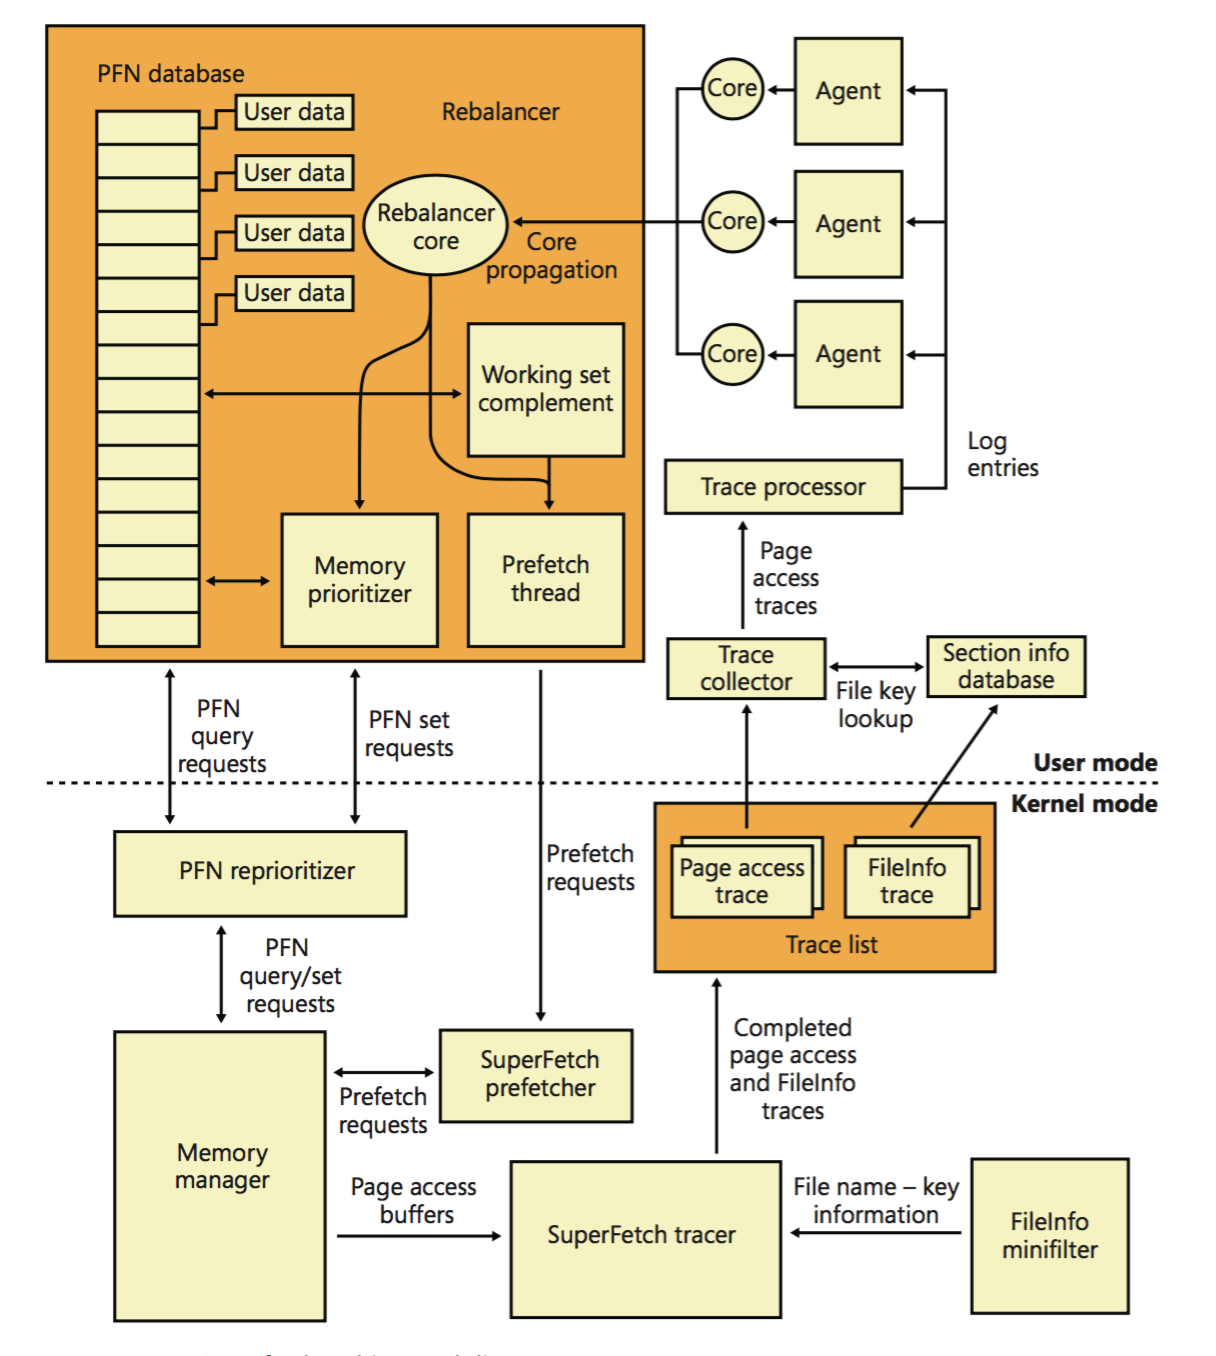
\includegraphics[scale=0.5]{./superfetch.eps}
\caption{SuperFetch Architectural Diagram from Windows' Internals Volume 2}
\end{figure}

True to NT's hybrid kernel design, the SuperFetch service runs partially in user space and partially in kernel space. It keeps a database of past program memory accesses and attempts to prognosticate what pages will be required in the future. Because SuperFetch learns from a user's interactions with Windows, if new software or a large system change like a new service pack is installed it will take a while to be retrained by the user. To combat this, new service packs come with a bundle of trace training data used to update the SuperFetch database so it doesn't have to be retrained.

Windows keeps a system thread running called the Balance Set Manager. Once every second, the balance Set Manager wakes up and decides which pages need to be swapped to disk. Alternatively this system thread can be awoken by a signal from the kernel's memory manager. The Balance Set Manager does not actually perform the swapping itself, instead it dispatches another kernel thread known as the Working Set Manager.

\section{Conclusion}
One of a kernel's most important jobs is allocating and sharing resources among programs. The single resource which absolutely every process needs is memory. Every structure and every cache which a kernel uses to more fairly allocate resources or provide them more quickly requires more memory. This constant pressure requires elaborate schemes to provide isolation, security, to share certain memory resources, and to ensure that every process gets its fair share.

\clearpage
\printbibliography

\clearpage

\begin{appendices}


\end{appendices}
\end{document}
\bibliography{bib.bib}
\bibliographystyle{IEEEtran}
